% Created 2020-03-24 Tue 13:27
% Intended LaTeX compiler: pdflatex
\documentclass[11pt]{article}
\usepackage[utf8x]{inputenc}
\usepackage[T1]{fontenc}
\usepackage{graphicx}
\usepackage{grffile}
\usepackage{longtable}
\usepackage{wrapfig}
\usepackage{rotating}
\usepackage[normalem]{ulem}
\usepackage{amsmath}
\usepackage{textcomp}
\usepackage{amssymb}
\usepackage{capt-of}
\usepackage{hyperref}
\usepackage{minted}
\author{Jakub Zárybnický (xzaryb00@stud.fit.vutbr.cz)}
\date{\today}
\title{Hledání genů}
\hypersetup{
 pdfauthor={Jakub Zárybnický (xzaryb00@stud.fit.vutbr.cz)},
 pdftitle={Hledání genů},
 pdfkeywords={},
 pdfsubject={},
 pdfcreator={Emacs 26.3 (Org mode 9.1.9)}, 
 pdflang={Czech}}
\begin{document}

\maketitle

\section{Identifikace otevřeného čtecího rámce}
\label{sec:orgbdffc33}
Prostřednictvím nástroje \href{https://www.ncbi.nlm.nih.gov/orffinder/}{ORF Finder} vyhledejte nejdelší otevřený rámec (ORF) na
genomové sekvenci bakteriofágu 3A ze souboru \href{./bacteriophage\_3A.txt}{bacteriophage\(_{\text{3A.txt}}\)}. Protein
kódovaný daným ORF porovnejte prostřednictvím blastp s proteiny dostupnými v
databázi nr.

\begin{enumerate}
\item Určete nejdelší ORF (nejdelší ORF obvykle bývá ten správný).
\begin{enumerate}
\item 99\% shoda s ORF001 Staphylococcus aureus
\end{enumerate}
\item Je sekvence genu odpovídající nejdelšímu ORF kompletní (odhadněte na základě
analýzy blastp - lze spustit přímo z nástroje ORF Finder)?
\begin{enumerate}
\item E = 0 pro alignment s NC\(_{\text{007053.1}}\) (9430-10989)
\end{enumerate}
\end{enumerate}

\section{Změna otevřeného čtecího rámce vlivem mutace - Single nucleotide polymorphism (SNP)}
\label{sec:orga5153e3}
Mutace protein-kódující sekvence může změnit otevřený čtecí rámec (vznik /
poškození na start / stop kodónu). Jedním z mnoha příkladů může být varianta
hemoglobinu nazývaná \emph{Constant Spring}. Tato varianta byla poprvé objevena na
Jamaice a od standardní varianty se liší svoji délkou. Více podrobností ohledně
této mutace můžete prostudovat v databázi OMIM pod identifikátorem \href{http://omim.org/entry/141850}{141850}.

\begin{enumerate}
\item Stáhněte z databáze GenBank standardní variantu nukleotidové sekvence
proteinu \href{http://www.ncbi.nlm.nih.gov/nuccore/NM\_000517.4}{HBA2 homo sapiens - mRNA} (stahujte celý záznam ve formátu
FASTA). Použijte nástroj \href{https://www.ncbi.nlm.nih.gov/orffinder/}{ORF Finder} ke zjištění délky ORF.
\begin{enumerate}
\item nt=429, aa=142
\end{enumerate}
\item Stáhněte nukleotidovou sekvenci varianty hemoglobinu \href{./constant\_spring\_rna.txt}{Constant
Spring}. Použijte nástroj \href{https://www.ncbi.nlm.nih.gov/orffinder/}{ORF Finder} ke zjištění délky ORF.
\begin{enumerate}
\item nt=522, aa=173
\end{enumerate}
\end{enumerate}

\section{Predikce genů založená na analýze sekvence a sekvenčních signálů}
\label{sec:orgaa22ef8}
Sekvenční analýza může poskytnout relevantní informace využitelné pro predikci
genů. Pro řešení následujích úloh využijte sadu nástrojů zvanou \href{http://emboss.bioinformatics.nl}{EMBOSS
toolbox}. Experimentování provádějte, není-li uvedeno jinak, na nukleotidové
sekvenci proteinu HBA2 ze souboru \href{./protein\_HBA2.fasta}{protein\(_{\text{HBA2.fasta}}\)}. Pro lehčí hledání odpovědí
na níže uvedené otázky si přečtěte něco o \href{https://cs.wikipedia.org/wiki/Methylace\_DNA}{methylaci DNA} a \href{https://en.wikipedia.org/wiki/CpG\_site\#CpG\_islands}{CPG ostrůvcích}.

\begin{enumerate}
\item \href{http://emboss.bioinformatics.nl/cgi-bin/emboss/compseq}{CompSeq}: spočítejte frekvenci výskytu jednotlivých dinukleotidů v
sekvenci. Má dinukleotid CG jinou než očekávanou frekvenci výskytu? Pokud
ano, zdůvodněte proč.
\begin{enumerate}
\item frekvence 3.91\% je pouze 62.5\% z očekávané 6.25\%, CpG se (dle wiki) u
obratlovců vyskytuje méně z důvodu možné degradace cytosinu na thymin.
\end{enumerate}
\item \href{http://emboss.bioinformatics.nl/cgi-bin/emboss/cpgplot}{CpgPlot}: Identifikujte oblasti CpG ostrůvků a vysvětlete, jak lze znalost o
těchto oblastech využít pro hledání genů.
\begin{enumerate}
\item V HBA2 se vyskytují tři regiony s CpG ostrůvky, na začátku, uprostřed a
cca v 75\%. Dle wiki jsou CpG ostrůvky většinou následované začátkem genu
\end{enumerate}
\item \href{http://emboss.bioinformatics.nl/cgi-bin/emboss/dreg}{Dreg}: Identifikujte polyadeninové signály v sekvenci \href{http://www.ncbi.nlm.nih.gov/nuccore/NG\_000006.1}{NG\(_{\text{000006}}\)} (stahujte celý
záznam ve formátu FASTA). Nejčastějšími polyadeninovými signály jsou AATAAA a
ATTAAA. Jak často se v sekvenci vyskytují?
\begin{enumerate}
\item Sekvence AATAAA celkem 39x
\item Sekvence ATTAAA celkem 13x
\end{enumerate}
\end{enumerate}

\section{Identifikace strukturních genů pomocí aplikace GeneMark}
\label{sec:orgbc89d3e}
V části bakteriální sekvence \href{./heliobacillus\_mobilis.txt}{Heliobacillus mobilis} proveďte prostřednictvím
aplikace \href{http://exon.biology.gatech.edu/gmchoice.html}{GeneMark} vyhledání strukturních genů. Používejte výchozí nastavení
vstupního formuláře, ve kterém změňte druh na "Bacillus\(_{\text{subtilis}}\)\(_{\text{168}}\)" (položka
"Select Species").

\begin{enumerate}
\item Kolik ORF bylo detekováno na přímém vlákně?
\begin{enumerate}
\item 15 ORF na přímém vlákně, 2 na komplementárním
\end{enumerate}
\item Lokalizujte ribozomální vazebná místa (RBS). Za konsensuální model pro E.Coli
je považována sekvence \emph{AAGGAG}, která je umístěna typicky 4-12 nukleotidů před
start kodónem. Tato RBS najděte pomocí utility \href{http://emboss.bioinformatics.nl/cgi-bin/emboss/dreg}{Dreg} z balíku
\href{http://emboss.bioinformatics.nl}{EMBOSS}. Regulární výraz sestavte tak, že:

\begin{itemize}
\item na první pozici RBS může být A, C nebo G
\item na druhé až páté pozici RBS může být pouze sekvence AGGA
\item na šesté pozici RBS může být A nebo G
\item mezera mezi RBS a start kodónem může být 4-12 nukleotidů
\end{itemize}

Jak vypadá Vámi použitý regulární výraz? Kolik jste našli odpovídajících
výskytů? Kolik z nich je relevantních (tj.  nacházejících se v blízkosti ORF
predikovaného pomocí GeneMark)?
\begin{enumerate}
\item\relax [ACG]AGGA[AG].\{4,12\}ATG
\item 10 výskytů
\item pozice RBS na 582, 6188, 7126, 8821, 12869
\end{enumerate}
\end{enumerate}

(GeneMark na přiložené adrese \url{http://exon.biology.gatech.edu/} nefunguje,
používám \url{http://opal.biology.gatech.edu/GeneMark/gm.cgi})

\begin{center}
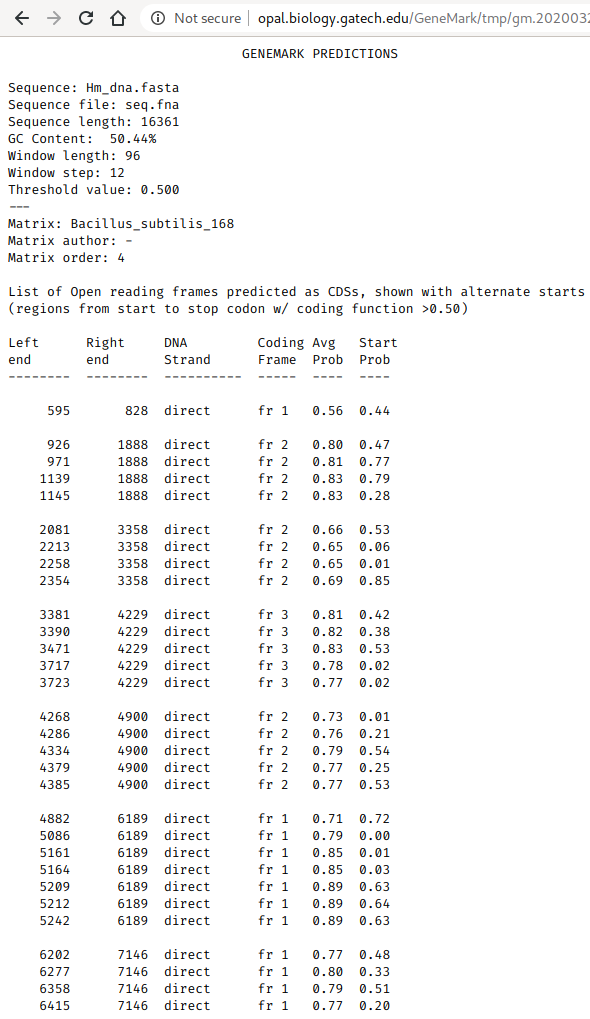
\includegraphics[width=1.2\linewidth]{./bif-5-genemark.png}
\end{center}

\section{Predikce operonů}
\label{sec:org5ce5dad}
Operony jsou sekvencí nukleotidů, resp. řadou po sobě jdoucích genů v
bakteriálním chromozomu, které mají společný promotor a jsou regulovány
společným operátorem a exprimovány najednou. Tyto geny kódují většinou enzymy
zapojené v jedné metabolické dráze.

Predikujte operony nad bakteriální sekvencí \href{./heliobacillus\_mobilis.txt}{Heliobacillus mobilis} pomocí \emph{40bp
pravidla}: Pokud je intergenová vzdálenost dvojice nepřímo transkribovaných genů
menší než 40 párů bází, potom je tato dvojice nazývaná operon.

\begin{enumerate}
\item S využitím výstupu genové predikce GeneMarku z předchozí úlohy určete první
operon na přímém vlákně.
\begin{enumerate}
\item Pokud uvažuju pouze s výstupen GeneMark, tak je to 2081 (následují geny na
3381 a 4268).
\end{enumerate}
\end{enumerate}
\end{document}